\documentclass[12pt]{article}
\usepackage[utf8]{inputenc}
\usepackage[T1]{fontenc}
\usepackage{booktabs}
\usepackage{graphicx}
\usepackage{csvsimple}
\usepackage{hyperref}
\usepackage{xcolor}
\usepackage{url}



\title{\textbf{ÉCOLE POLYTECHNIQUE FÉDÉRALE DE LAUSANNE \\ Laboratory for Reactor Physics and Systems Behaviour (LRS) \\ Research Internship report: 
\\ A Parametric study of various Lattice code computational models of Pin-Cells and Reactor Assemblies for a selection of input parameters}}
\author{\textbf{Alexandre Stuart} \\ McGill University Department of Physics\\[0.5cm]  Under the supervision of Prof. Mathieu Hursin}
\date{September 2021}
\usepackage[margin=1in]{geometry}
\usepackage{graphicx}
\usepackage{subcaption}
\begin{document}

\maketitle
\section{Introduction}

Generating around 10\% of the world's electricity and around 24.8\% of the world's low carbon electricity (2021), the world's fleet of around 440 operational nuclear power reactors are some of the most important pieces of energy infrastructure. As such, it is paramount to be able to model the neutronic behaviour of nuclear reactions taking place in these reactors for a number of different variables such as fuel composition, fuel temperature and neutron leakage to name a few. In the mid 1960s, the first lattice physics codes were developed (WIMS-Winfrith Improved Multigroup Scheme, 1966) which gathered all the processes required to obtain cross section data in a variety of computational modules and added a two dimensional calculation, which allowed to analyse a two-dimensional fuel assembly (a 2D geometry is one that has boundaries along two axes, lattice codes code the z-axis as infinitely tall, therefore there is no boundary along this axis), in contrast to the mainstream code of the time that only allowed for pin-cell calculations \cite{Knott2010}. These new 2-D geometries allowed to take into account neutronic interactions between pins, water gaps, channel walls etc. 

The general structure of a lattice code input/output scheme is the following: the code takes a microscopic cross section standard library and a reactor lattice, a geometry as inputs and through its variety of computational modules and options, solves the  Boltzmann Transport Equation (BTE) with deterministic methods such as the Collision Probability (CP), Method of Characteristics (MOC) and Interface Current (IC) methods used in this project which require its Multi-Group discretization \cite{ghasabyan2020validation}. 

The differential form of the Multi-Group BTE is the following \cite{ligou1997introduction}:

\begin{equation}
    \Omega \cdot \nabla \phi_g(r, \Omega) + \Sigma_g(r)\phi_g(r, \Omega) =Q_g(r, \Omega)
\end{equation}

with group-average values of the flux defined as: 

\begin{equation}
    \phi_g(r, \Omega) = \int_{u_{g-1}}^{u_g} \! \phi(r, u, \Omega) \, \mathrm{d}u
\end{equation}
\begin{equation}
    Q_g(r, \Omega) = \int_{u_{g-1}}^{u_g} \! Q(r, u, \Omega) \, \mathrm{d}u
\end{equation}
 
 The characteristic form of the Multi-Group BTE is given by:
 
 \begin{equation}
     \frac{d}{ds}\phi_g(r + s\Omega, \Omega) + \Sigma_g(r + s\Omega)\phi_g(r + s\Omega, \Omega) = Q_g(r + s\Omega, \Omega)
 \end{equation}
 
 The integral form of the Multi-Group BTE is written as: 
 \begin{equation}
     \phi_g(r, \Omega) = \int_0^{\infty} \! e^{-\tau_g(s)}Q_g(r - s\Omega, \Omega) \, \mathrm{d}s
 \end{equation}
 
 with the optical path $\tau_g(s) =  \int_0^s \! \Sigma_g(r + s' \Omega) \, \mathrm{d}s'$  

Lattice codes give the solution of this equation as an eigenvalue problem. In this project, the lattice code gave the eigenvalue to be the effective multiplication factor 

\begin{equation}
    K_{eff} = \frac{production}{absorbtion+leakage},
\end{equation}

which in other words is the ratio between neutrons produced, and neutrons lost. It was assumed that there was no neutron leakage, so $K_{eff} = K_{inf}$. The BTE solution also gives a neutron flux distribution, which itself can be inputted through modules to find macroscopic cross sections and thus reaction rates, fuel depletion(burnup) and pin-power values. 

\begin{figure} [htb!]
\centering
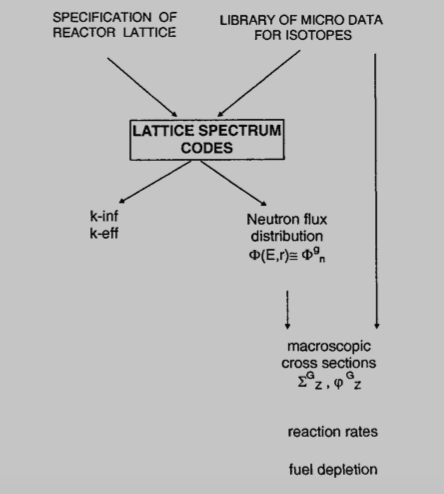
\includegraphics[scale=0.4]{Figures/Lattice code diagram.png} 
\caption{General lattice code input/output scheme}
\end{figure}

\section{Motivation}

The goal of this project was to assess the impact on output variables of updating input parameters on different existing lattice code computational models of neutron transport in nuclear fuel under irradiation. This assessment could lead to refinements to the existing models or the creation of more fitting models if necessary. Four models in total were studied, one model of a pin-cell, and three different computational models of an eighth of a Westinghouse designed 17 by 17 cell Pressurized Water Reactor (PWR) fuel assembly. Different variables were analysed depending on the type of model studied, namely the effective multiplication factor in the case of the pin-cell model, to which a study of pin-power values was added for certain fuel assembly models. In the case of the pin-cell model, the fuel and moderator temperatures were altered, as were the standard microscopic cross section standard libraries with respect to the type of library and the number of groups within the energy mesh in the library. In the case of the assembly models, these same parameters were altered on the most basic assembly geometry given, that is, an eighth of a 17x17 assembly with empty (water filled) guide tubes and no instrument thimble nor poisons (geometry pictured below in Fig. 3b, and again in Appendix A). The assembly models were then run on most of the other assembly geometries given in Appendix A, modifying all aforementioned parameters but mixture temperatures. These alterations follow the Consortium for Advanced Simulation of LWR (CASL) VERA Core Physics Benchmark Progression Problem Specifications \cite{godfrey2013vera} Problems 1 and 2 for the pin-cell and assembly calculations respectively, and results obtained were compared to the given problem solution. 


\section{Software}

\subsection{DRAGON Version5}

 DRAGON Version5 \cite{hebert2016dragon5}\cite{marleau2011user} is a lattice code developed since 1991 and owned by École Polytechnique de Montréal. DRAGON is free software and can be redistributed and modified under the terms of the GNU Lesser General Public License. Its structure is modular, with its computational modules written in Fortran 2003. This design allows for easy editing of the code. Its execution is controlled by the CLE-2000 Supervisor. DRAGON is designed to perform standard lattice code  operations that simulate the neutronic behavior of a unit cell or fuel assembly and can be used to solve the BTE. Namely: interpolating a predefined microscopic cross section standard library containing all the isotopes to be used, performing multidimensional geometry resonance self-shielding calculations, performing multigroup and multidimensional neutron flux calculations with or without leakage, performing transport-transport or transport-diffusion equivalence calculations, editing of condensed and homogenized nuclear properties, and finally, performing isotopic depletion calculations. DRAGON contains various distinct methods to carry out each of these calculations, which are represented by different modules to choose from while writing the DRAGON input data structure. 

A DRAGON input data structure obeys a strict format dictated by the GAN generalized driver. This means that any structures, structure storage locations and modules   are defined before any execution related code.  The modules are then successively called and information is fed from one module to the next, where the execution ends at the END: keyword. The input data structure is written in this same order. 

In this project, DRAGON was used to solve the BTE on pincells and assemblies. To do so the following modules can be used in the given order:
 
\begin{itemize}
    \item The LIB module is used to define the microscopic cross section standard library used and the isotopic mixtures used in each subsection of the cells in the model. \item The GEO module defines the geometry of the cell and where each of the mixtures defined within the previous module are to be located within the geometry. This module can be replaced with the G2S module in the case of gigogne geometries. \item For any of the IC, MOC or CP methods a tracking module is required to analyze the predefined geometry. It performs zone numbering operations, volume and surface area calculations and generates integration lines. The tracking modules used in this project are the EXCELT, MCCGT and SYBILT modules, which are used to perform CP, MOC and IC tracking respectively in the case of 1-D geometries. The MCCGT must call one of the EXCELT, NXT or SALT module by definition. In the case of 2-D and 3-D geometries, the NXT module can be used instead of EXCELT for IC tracking and the SALT module can be used to perform CP and MOC tracking in 2D. SALT takes an input that can be built with the G2S module. \item The USS (Universal Self-Shielding) module accounts for the self-shielding effects occuring due to the presence of resonant isotopes. \item The ASM module prepares collision probability or assembly matrices for the FLU module \item The FLU module solves the BTE for the fluxxes. \item The EDI module is used to save the nuclear properties on a defined output file \item The UTL module can be used to perform tasks unrelated to reactor physics. E.g. can be used to create a block of information in DRAGON. 
\end{itemize} 

 \subsection{Models used}
 
 During this project, four different DRAGON template input structures (\href{https://github.com/alex-stuart/LRS_internship_repo/tree/main/dragon/filesToRun/x2mFiles}{\color{blue}{here}}) were used.  

The first is a model of the unit pincell given in problem 1 of CASL \cite{godfrey2013vera} shown in diagram below. All isotopic compositions are given in Table P1-4 in Appendix A. There are therefore four mixtures defined in the LIB module which are used in the GEO module, which defines the geometry of the cell as concentric circles of different radii within a square. The space between these shapes is filled with the mixtures defined within the previous module. In the libraries used, helium was found to cause errors in the model and thus the fuel-clad gap was removed from the model, the area of this gap was added to that of the cladding mixture. 
The DRAGON5 model uses MOC tracking for a 1D geometry, and thus the input includes MCCGT tracking.

\begin{figure}[h]
\centering
\subfloat[\label{fig:subassembly}]{%
  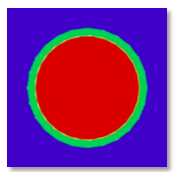
\includegraphics[scale=0.6]{Figures/Pincell diagram.png}}
\hspace{0.01cm}
\subfloat[\label{tab:subkey}]{%
      \begin{tabular}{r|l}
        Rod Pitch (width) & 1.26cm\\
        Fuel pellet radius & 0.4096cm\\
        Inner clad radius & 0.418cm\\
        Outer clad radius  & 0.475cm\\
      \end{tabular}}
\caption{Pincell diagram and specifications}
\label{fig:subassemandkey}
\end{figure}

This pincell model is run for testcases 1A-1D in table P1-5. Testcase 1E was run but presented too much of a discrepancy and was discarded.

\begin{figure} [htb!]
\centering
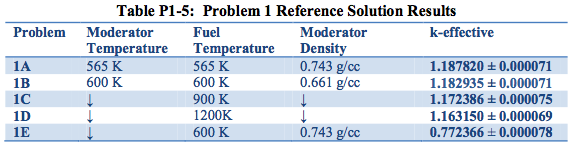
\includegraphics[scale=0.7]{Figures/CASL P1 resultsTable.png}
\end{figure}

 The three others are three distinct models of an eighth of a template 17 by 17 fuel cell assembly. One such assembly geometry (geometry 2A-2D) is depicted in Figure 3b. 
 
 \begin{figure} [htb!]
\centering
\begin{subfigure}{.5\textwidth}
  \centering
  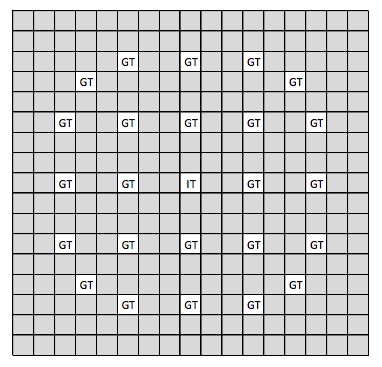
\includegraphics[scale=0.4]{Figures/Assembly Geometry 1.png}
  \caption{Assembly diagram}
  \label{fig:sub1}
\end{subfigure}%
\begin{subfigure}{.5\textwidth}
  \centering
  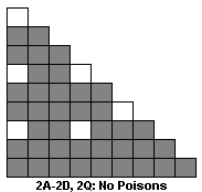
\includegraphics[scale=0.7]{Figures/1:8 assembly diagram .png}
  \caption{1/8 Assembly diagram}
  \label{fig:sub2}
\end{subfigure}
\caption{1 and 1/8th of a 17 by 17 Assembly respectively}
\label{fig:test}
\end{figure}
 
 This assembly geometry has 3.1\% enriched fuel in all fuel rods. Also note that while all of the empty tubes are depicted as white squares in the 1/8th Assembly diagrams, as can be seen in figure 3a there are two distinct types of empty tubes. There is an Instrument Tube, IT in the centre of the assembly designed to hold an instrument thimble and Guide Tubes, GT placed radially around the Instrument Tube (as can be seen in figure 3a), designed to hold different types of rods, such as AIC (Silver-Indium-Cadmium) and $B_4C$ (Boron Carbide) control rods, or discrete burnable neutron absorbers such as Pyrex. The assembly output data for the entire 17 by 17 assembly can be extrapolated from symmetry.

The first assembly model is a classical single level calculation scheme. This scheme is based on the use of a cross-section library in DRAGLIB format, a SHEM295 energy mesh, two geometries and their respective trackings, a self shielding geometry used with the IC method (Geo\_SS\_1L.c2m) where some cell regions are merged together to save CPU costs and a flux-solution geometry used for the BTE solution with the MOC method (Geo\_N2.c2m). The required geometries and library (MIX\_UOX\_1L.c2m) are written in separate files and are imported in the DRAGON5 running script (.x2m file). As such, the SYBILT module is used on the self-shielding geometry and the SALT, MCCGT modules are used on the flux solution geometry. the driver then calls the self shielding module USS on the self-shielding tracking. In this call there are only eight cell regions, the CELL C1-C8 regions in (MIX\_UOX\_1L.c2m) that are reused for all other mixtures in the assembly below in the mixture file. The ASM, FLU and EDI modules are then called on the flux calculation tracking, in that order. In this project the burnup was not run.

Due to its use of MOC, this method can handle larger assembly problems with greater accuracy at the expense of longer calculation times in comparison to the second model.

The second model is based on the two level calculation scheme written in \cite{canbakan2015accuracy}. It uses two sets of isotopic mixtures, three geometries and two energy meshes defined as follows:

Mixtures:
The first set of mixtures is used for self-shielding and first level BTE solution with the IC method, while the second is used for the second level BTE solution with the MOC method. This mixture can also be used to calculate the Bateman equation (link bateman) solution by performing burnup, but this was not studied during this project. These mixtures are all part of the same file, Mix\_UOX.c2m. Note that the isotopic content of the mixtures is again recovered from a cross-section library in DRAGLIB format. This isotopic content is defined for a limited set of first level mixtures.

Geometries:
-A self-shielding geometry used with the IC method (Geo\_SS.c2m). Moderator regions are not submeshed and some fuel regions are merged together to save costs.
-A first level geometry used for the BTE solution with IC method (Geo\_N1.c2m). This geometry is similar to the previous geometry but moderator regions are better discretized.
-A second level geometry used for the BTE solution with the MOC method (Geo\_N2.c2m). This is the same geometry as the flux solution geometry in the one level scheme. 

The scheme follows a similar structure to the single level scheme (1L). The tracking for the self-shielding geometry is the same as in 1L and the first level geometry tracking is a repetition of this. Note that the resonance self-shielding calculation is performed over 295 energy groups and for a limited set of first-level mixtures. The tracking for the second level geometry is the same as the flux solution tracking from 1L, as expected. The first flux calculation is then performed using the ASM, FLU modules and the EDI module performs a condensation of first level cross sections over the second-level energy mesh. The superhomogenization equivalence module (SPH) is then called to preserve reaction rates from the pre-condensation calculation. The microlib is expanded from the first-level mixture to the second-level mixture with Mult\_LIBEQ.c2m. and finally, the BTE is solved with the MOC by using the ASM, FLU modules as before. 

The code for these first two assembly DRAGON5 models was derived from the Assembly A (37 first level and 161 second level mixtures) code found on the \href{https://github.com/tumregels/msca/tree/master/Dragon}{\color{blue}{github page}} of L.Ghasabyan's validation study. \cite{ghasabyan2020validation}

The third model is a simplistic modification of the two level calculation scheme to allow for extremely rapid computation times. That is, the second level flux calculation was removed and the output of the first level is saved in the output file. 

\begin{figure} [htb!]
\centering
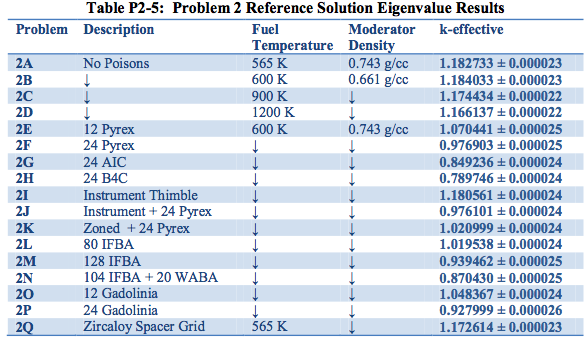
\includegraphics[scale=0.7]{Figures/CASL P2 resultsTable.png}
\end{figure}

Each of these three assembly template input structures were run over test cases 2A-2D in Table P2-5, taking for standard library the DRAGLIB ENDF70\_295 to compare the validity of these three assembly models, both in terms of the effective multiplicative factor ($K_{eff}$) results and the derived pinpower results and corresponding maps. This choice of cross-section library is made as the CASL reference solutions are calculated with the ENDF/B-VII.0 CE (ENDF70) cross section library while the one-level and two-level assembly models were designed to take as input a DRAGLIB format 295 energy group library as mentioned above. 

The simple assembly models were also run over some of the test cases in 2E-2P, in particular E, G, H I, O, P. These are based on a variety of different 17 by 17 assembly geometries which can be found in Appendix A, with different pins in the guide tubes namely Pyrex, AIC and $B_4C$ control rods in the guide tubes and an instrument thimble in the instrument tube. In Geometry 2K in this image, the fuel is radially zoned, i.e. the fuel is denser in most of the assembly,excluding the very centre and the four corners. Geometries 2L-2P in this image have empty guide and instrument tubes but some fuel rods are replaced with burnable absorbers such as Integral fuel (IFBA), Wet Annular (WABA) and Gadolinia Integral (Gad) to optimize assembly reactivity control and power distribution management. Note, an IFBA rod is a standard $UO_2$ with a $10\sigma m$ coating of $ZrB_2$, while a Gadolinia Integral burnable absorber rod has the same geometry as a $UO_2$ fuel rod but a different fuel mixture including Gadolinium. The other various rods used are shown with their specifications in Appendix A along with their isotopic compositions in Table P2-4. This set of different assemblies was run for all of the libraries defined in the next section. All of the different corresponding input files used can be found \href{https://github.com/alex-stuart/LRS_internship_repo/tree/main/dragon/filesToRun}{\color{blue}{here}}.

\subsection{Libraries}

The microscopic cross section standard libraries used were taken from the list of preexisting libraries on the LRS server. Some libraries in this list were discarded due to difficulty finding the correct isotope local names (ID), namely the I\_172W and I\_69W IAEA libraries. These isotope IDs were obtained by running the functional DRAGON5 code on the libraries to obtain the following ID information as well as using the WIMSID rosetta stone (wimsid.dms). Some libraries were also discarded for having identical information and returning identical results (FAN\_REP=J40\_172W, J41\_172W=J42\_172W)

DRAGON5 takes multiple different library formats as input to the LIB module. In this project, two different input formats were used; DRAGLIB and WIMS-D4. In the plots in the following section, all WIMS-D4 libraries have a W at the end of their name and all DRAGLIBS do not. These are two of the six formats supported by DRAGON5. Each of these two different library types were created by the dragr and wimsr modules respectively from three different library formats JEFF (Joint Evaluated Fission and Fusion file), ENDF/B (Evaluated Nuclear Data File) and JENDL (Japanese Evaluated Nuclear Data Library), which are not directly supported by DRAGON5. As mentioned above the IAEA libraries provided were not run. The dragr and wimsr modules can be found in the NJOY-2012 source released by LANL \href{https://www.polymtl.ca/merlin/pynjoy2012.htm}{\color{blue}{here}}. 

In the plots below, all standard libraries are given names starting with J3 for JEFF, E or ENDF for ENDF/B and J4 for JENDL libraries, followed by the standard library version, an underscore and finally the number of energy groups.

The list of libraries that were run by DRAGON5 and related information can be found \href{https://github.com/alex-stuart/LRS_internship_repo/tree/main/dragon/Libs}{\color{blue}{here}}.

\subsection{Scripts used}

\href{https://github.com/alex-stuart/LRS_internship_repo/tree/main/dragon/scripts}{\color{blue}{Python scripts}} were used to run the various DRAGON models in a sequential manner and to extract the $K_{eff}$ values while \href{https://github.com/alex-stuart/LRS_internship_repo/tree/main/MatLab}{\color{blue}{Matlab scripts}} were used to extract fuel pin-power outputs. A Shell script (\href{https://github.com/alex-stuart/LRS_internship_repo/blob/main/bin/rdragon5}{\color{blue}{rdragon5}}) was provided to run DRAGON5. This script was copied and modified to allow for the use of different input files and different output name and locations (\href{https://github.com/alex-stuart/LRS_internship_repo/blob/main/bin/rdragon6}{\color{blue}{rdragon6}}).

\section{Parametric studies}

\subsection{Effective multiplication factor $K_{eff}$}

Running the pincell and simple assembly models on the aforementioned microscopic cross section libraries and testcases with the help of the scripts we obtain the following per hundred thousand differences between the $K_{eff}$ values outputted by DRAGON5 and the expected results given in CASL (calculated by the continuous energy (CE) Monte Carlo based transport tool KENO-VI) which are given in a csv table by the python scripts. In this results table geometry 2E (12 Pyrex) clearly stands out for giving very inaccurate results as all of the errors in pcm are O($10^4$). This was also true when running geometry 2F (24 Pyrex). From this we can say without much uncertainty that the representation of the Pyrex geometries used was very poor or incorrect. This result was therefore not plotted in the following graphs. All of the testcases above excluding case 2E are plotted in fig.13 in Appendix B. The libraries are noted above each set of cases, and the geometries are given in a legend below the plots. As seen in this figure the testcases 2G,H $K_{eff}$ values follow the same trends but are very far from a discrepancy of 0. This is again most likely due to poor or incorrect calculation models. These cases are not plotted in the following images to better focus on and observe library geometry trends.

\begin{figure} [htb!]
\centering
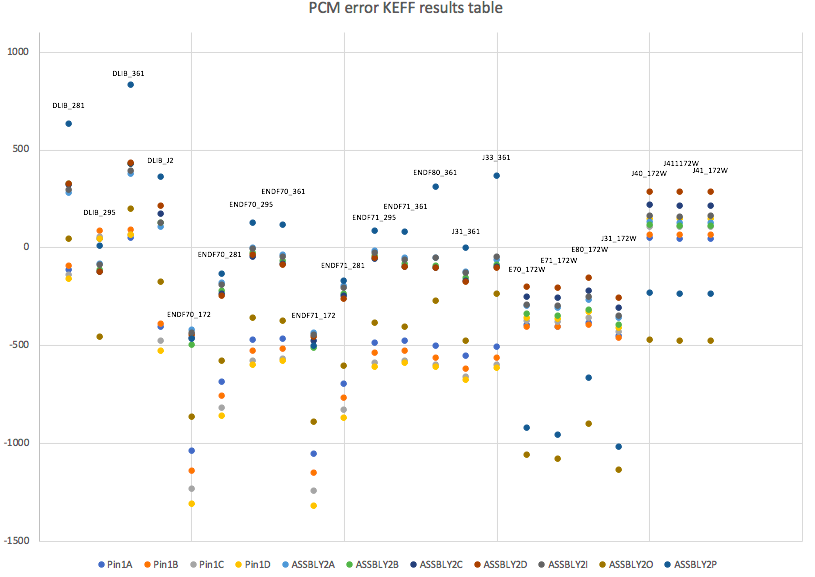
\includegraphics[scale=0.6]{Figures/allData-outliers2.png}
\caption{}
\end{figure}

As can be seen in fig 4, DRAGLIB type microscopic standard cross section libraries are much more accurate than the WIMSLIB type for some specific geometries and libraries, while WIMSLIB type libraries are more precise for most for most geometries with less variation between geometries and libraries. WIMSLIBs are also more accurate than DRAGLIBs for the same libraries and number of energy groups (172). In particular, WIMSLIBs are much more accurate for the pincell geometries, while for higher number of groups, all the other geometries represented are more accurately described by DRAGLIBs. Note that these trends are not accurate in the case of the non-standard libraries DLIB\_281, DLIB\_295, LIB\_361, which are much more precise, and on average, more accurate than the other DRAGLIBs. In fact, the most precise library is DLIB\_295. Given that the results given by CASL were calculated with ENDF70\_295 used, this is consistent, at the very least in terms of energy groups. More investigating should be done to find out if this is indeed an ENDF library.

\begin{figure} [htb!]
\centering
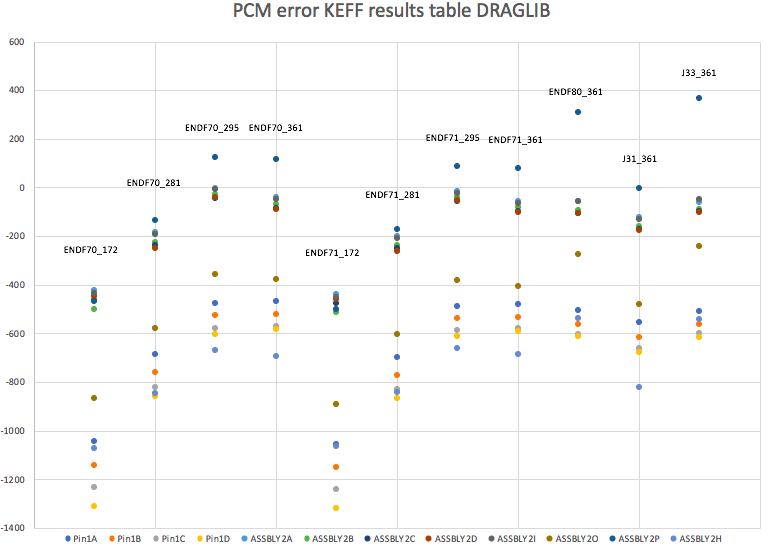
\includegraphics[scale=0.6]{Figures/DRAGLIB-DLIB2.png}
\caption{}
\end{figure}

As can be seen by isolating the results for the given DRAGLIB standard libraries in figure 5, the more energy groups in a library, the more accurate the results. This trend is especially true from 172 groups to 295 groups, as in the case of 361 energy groups the increase of accuracy is much less pronounced and in the case of assembly geometry $K_{eff}$ results are even slightly less accurate than for libraries with 295 energy groups. This is consistent with what is expected as the results given by CASL were calculated with ENDF70\_295. 

The data also indicates that in the case of DRAGLIBs, the newer the library, the more the groups of results (pins A, B, C, D, assemblies O, H in one, the rest in another) close in on themselves, and tighten in precision as the version of library increases. This is extremely obvious between ENDF71\_361 and ENDF80\_361 or J31\_361 and J33\_361. This could suggest that the pin models and the models for assemblies O and H are all poor calculations for the same reason. Note that in these two particular cases, assemblies 2P and 2O both increase significantly in $K_{eff}$ and do not follow this trend. In the case of Assembly 2P with J31\_361, the error is one of the smallest evaluated: -2.6293pcm, while with J33\_361 it has a value of 369.2138pcm. It may be of interest to investigate whether this is just coincidence or if the representation of Assembly 2P by the J33\_361 library is indeed correct.

These trends can also be observed in Figure 6 to a lesser extent, though here we see that the JENDL-4 library gives very different, more correct results to all the other libraries in the plot. 

Note that in Figures 5 and 6 the JEFF3.1 (2006) library gives results close (with a slightly larger error) to the ENDF-VII (2006) libraries, while in figure 6, the JEFF3.3 (2017) library gives results very close to the ENDF-VIII (2018). This makes sense given that these library major updates were created at around the same time to correct similar data. It might also be interesting to test lower energy group number DRAGLIB JEFF libraries to validate this further. 

\begin{figure} [htb!]
\centering
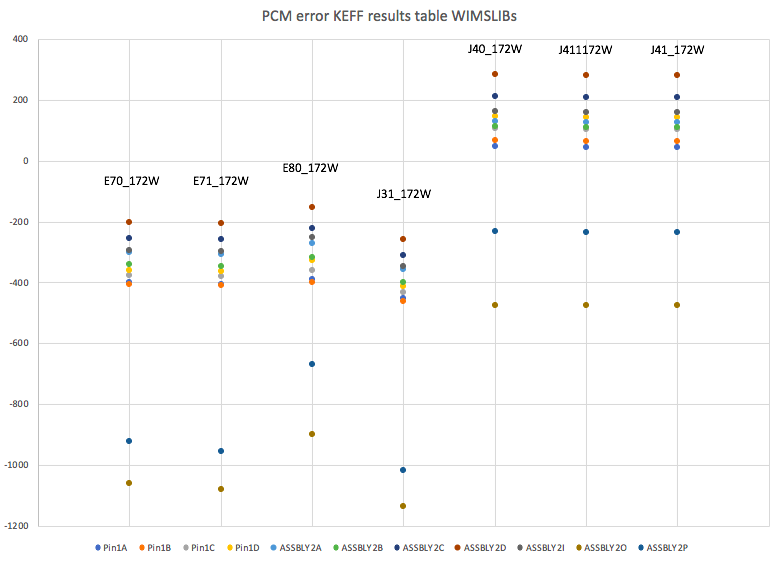
\includegraphics[scale=0.6]{Figures/WIMSLIBs2.png}
\caption{}
\end{figure}

As discussed above, the $K_{eff}$ values were calculated for the ENDF70\_295 library and assemblies 2A-2D with the three assembly calculations. These results are plotted in figure 7. As can be seen here, The simple calculation gives the exact same results as the first level calculation of the two level method as expected. This first level solution of the BTE is much more accurate than the second level solution or the BTE solution of the one level calculation. Also noticeable is that the second level solution of the BTE in the two level calculation has a smaller discrepancy than the solution of the one level calculation. This is consistent with figure 3.15 \cite{ghasabyan2020validation} (see Appendix B), where the discrepancy at zero burnup clearly has a greater magnitude in the negative direction in the case of the one level calculation. It could be beneficial to determine whether the two level $K_{eff}$ calculation represented in figure 3.15 is the first or second level solution of the BTE as this is not clear from \cite{ghasabyan2020validation}. One possible way this might be done is to run a few burnup steps and comparing the results of the two different results from the two level calculation with the trend observed in figure 3.15. In the case that the first level solution of the two level calculation is not the $K_{eff}$ discussed in \cite{ghasabyan2020validation} this would also provide information on how the quality of the simple calculation $K_{eff}$ results varies through burnup.

\begin{figure} [htb!]
\centering
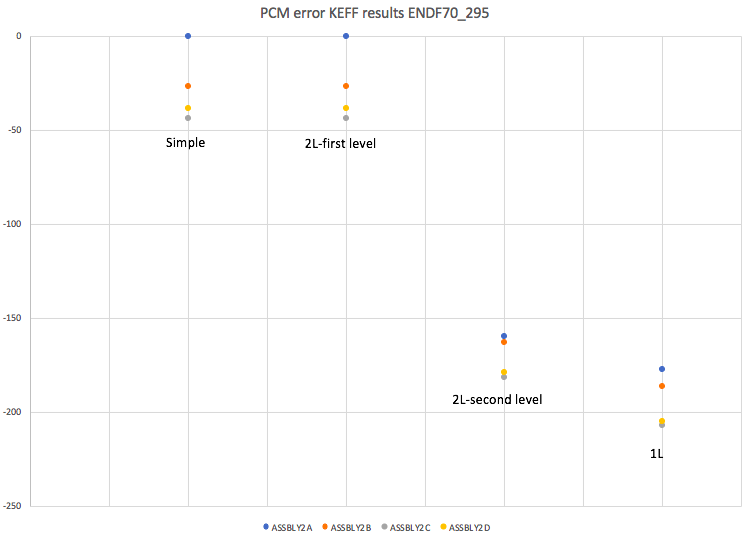
\includegraphics[scale=0.3]{Figures/ENDF70_295.png}
\caption{}
\end{figure}

From this it is clear that in the case of these four assemblies, The simplified method returns much better $K_{eff}$ results and is significantly faster than the two other more complex methods while the one level calculation returns the most discrepancy and is extremely slow. DRAGON5 takes approximately 1, 15 and 30 minutes to run the simple, 1L, 2L calculations respectively.

\subsection{Pin-Power}

As mentioned above, the Pin-powers were calculated for all pins in each assembly from 2A-D. These were plotted in terms of difference to the reference maps given in CASL on Pin-power percent discrepancy Maps. As explained above, since these four assemblies used the same number of mixtures, the same Assembly model, Assembly A could be used for all four. For other assemblies with different numbers of mixtures, one should try to adapt the other one and two level calculation assembly models provided in L.Ghasabyan's github repository \href{https://github.com/tumregels/msca/tree/master/Dragon}{\color{blue}{here}} (see also Table 2.1 in \cite{ghasabyan2020validation}). in the case of different mixtures for the fuel cells, one should make sure that there is the same number of fuel cells as before so as to respect the fuel regions given by the geometry and to allow each fuel cell to interact independantly from its neighbors.

Assembly 2A's maps can be seen in figure 8. From these it is observed that the one and two level (1L, 2L) solutions of the BTE, used to find the Pin-Power Maps are less accurate than the simple calculation. More explicitly, the maximum discrepancy in the one and two level calculations is a little less than 8\%, while that in the simple calculation is no more than 3\%. This is surprising given that in \cite{ghasabyan2020validation}, these same one and two level calculations gave a maximum discrepancy of 0.4\% at zero burnup when compared to SERPENT2 stochastic Monte Carlo code Calculations. This difference in results would be interesting to investigate further, however modifying the simple Pin-Power percent difference map seems to be a more promising path forward to obtain better Pin-Power results in a much shorter time.

\begin{figure}[htb!]

        \begin{subfigure}{.5\textwidth} % this sets the figure to be max half the width of the page
            \centering
            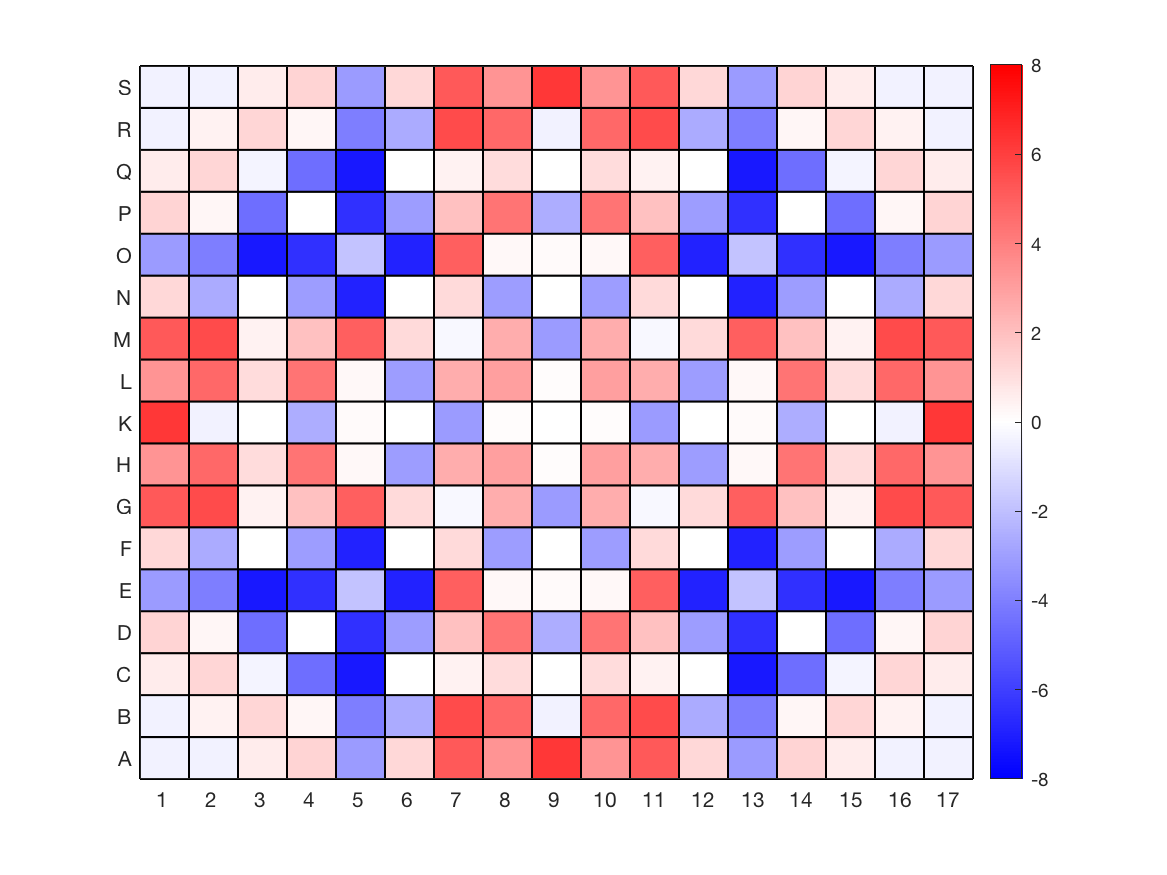
\includegraphics[scale=0.46]{Figures/2A_1L_pinpowerDiff.png} 
            \caption{Assembly 2A 1L Pin Power percent difference Map}
            \label{fig:sub-first}
        \end{subfigure}
        \begin{subfigure}{.5\textwidth}
            \centering
            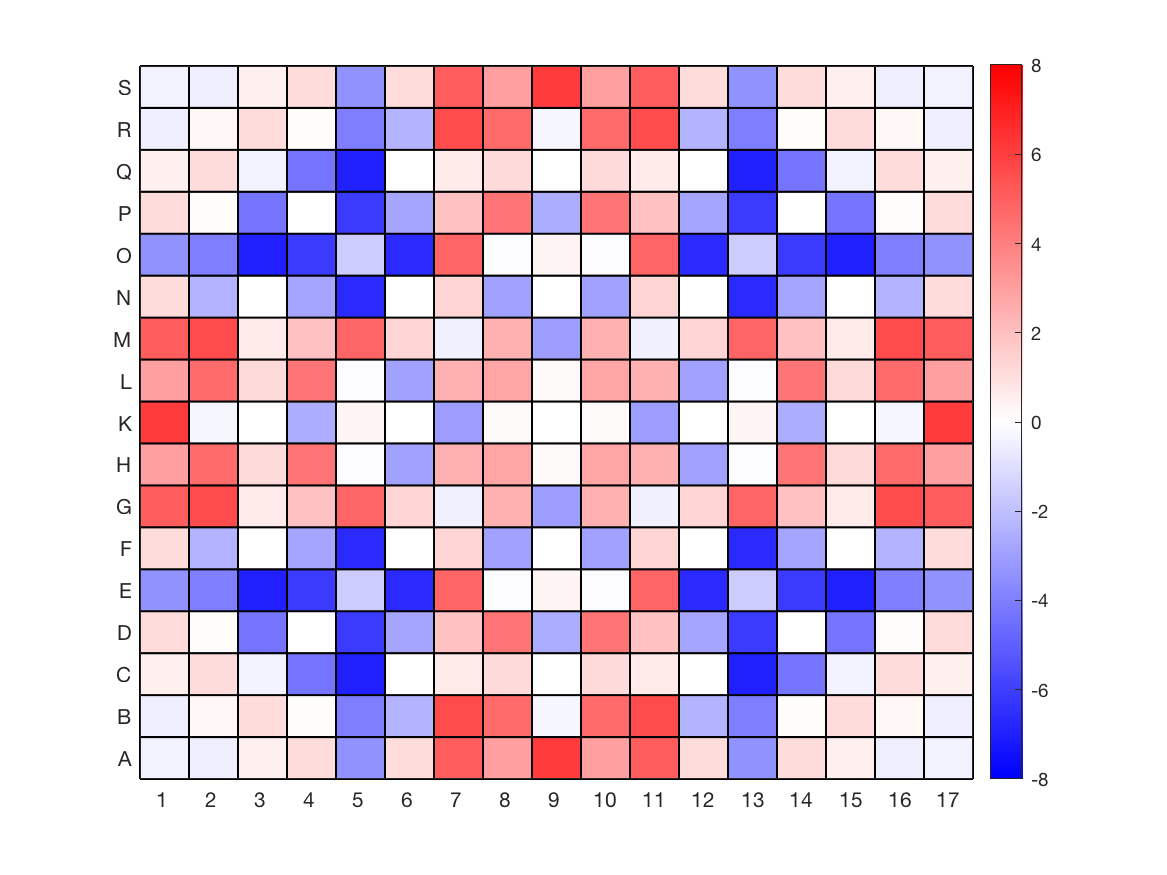
\includegraphics[scale=0.46]{Figures/2A_2L_pinpowerDiff.png} 
            \caption{Assembly 2A 2L Pin Power percent difference Map}
            \label{fig:sub-second}
        \end{subfigure}

        \label{fig:fig}
        \begin{subfigure}{\textwidth}
            \centering
            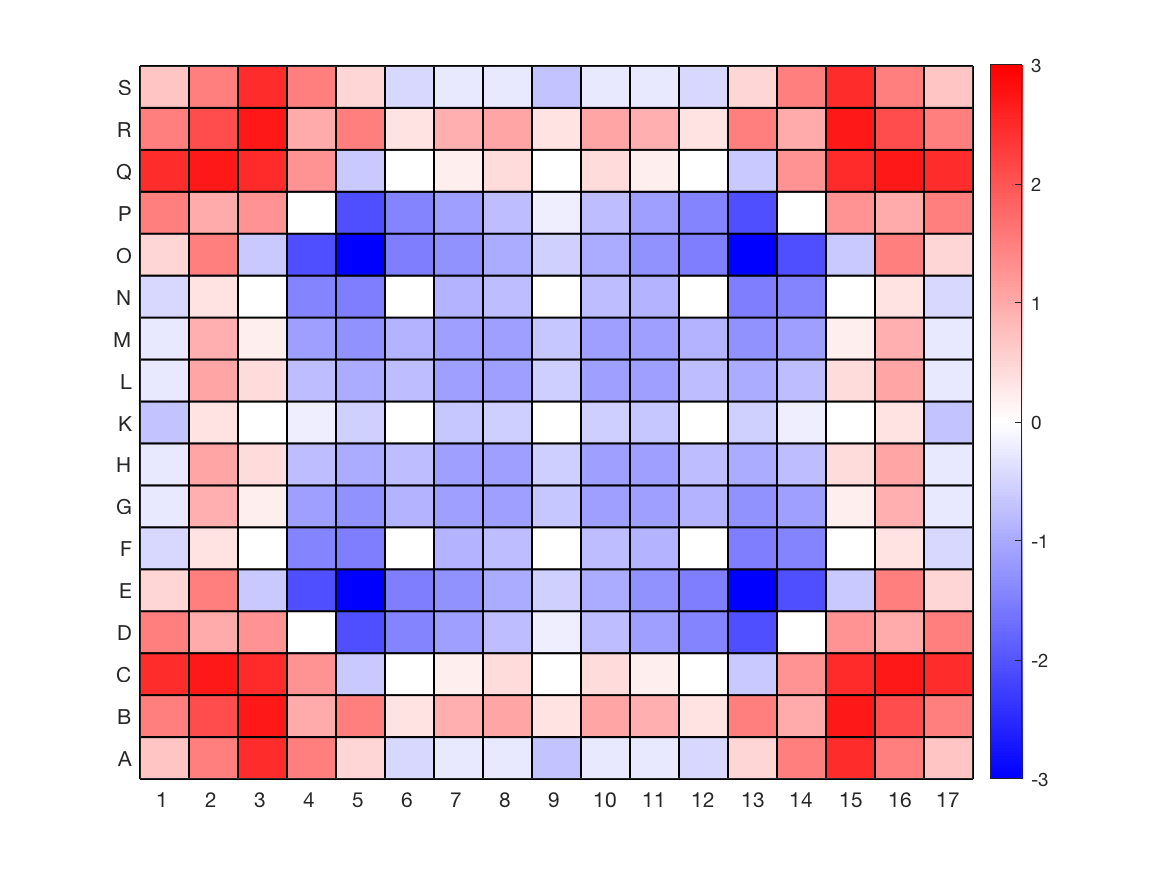
\includegraphics[scale=0.46]{Figures/2A_simple_pinpowerDiff.png}
            \caption{Assembly 2A Simple Pin Power percent difference Map}
            \label{fig:sub-firstA}
        \end{subfigure}
        \caption{Assembly 2A Pin Powers}
    \end{figure}

\newpage

The three other sets (Assemblies 2B-D) can be seen in Appendix A and the Pin-Power results are extremely close to those of assembly 2A. All of the raw Pin-Power results can be found \href{https://github.com/alex-stuart/LRS_internship_repo/tree/main/MatLab/Outputs}{\color{blue}{here}}.

\bibliographystyle{ieeetr}
\bibliography{MyBibliography}

\newpage
\thispagestyle{empty}
\appendix
\section{First Appendix: Input and expected output specifications, CASL Isotopic mixture compositions, pin-cell and assembly geometries}

\begin{figure} [htb!]
\centering
\begin{subfigure}{.5\textwidth}
  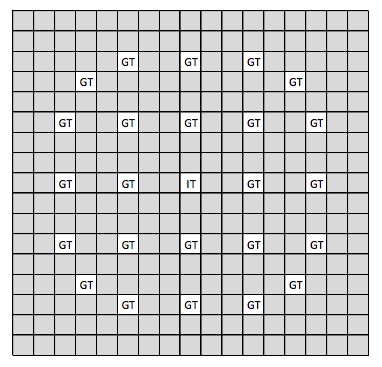
\includegraphics[scale=0.5]{Figures/Assembly Geometry 1.png}
  \label{fig:sub1}
\end{subfigure}%
\begin{subfigure}{.5\textwidth}
  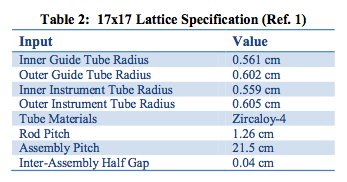
\includegraphics[scale=0.7]{Figures/Assembly Specs.png}
  \label{fig:sub2}
\end{subfigure}
\caption{Assembly lattice diagram and Specification}
\label{fig:test}
\end{figure}

\begin{figure}[htb!]
    \centering
    \subfloat{{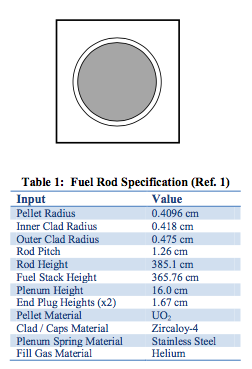
\includegraphics[width=4cm]{Figures/Fuel Rod specs:geom.png}}}%
    \qquad
    \subfloat{{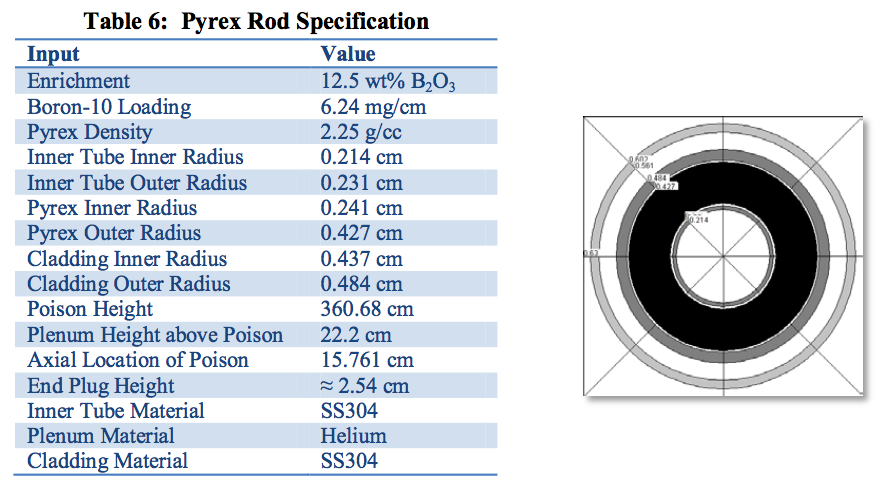
\includegraphics[width=10cm]{Figures/Pyrex specs:geom.png} }}%
\end{figure}

\newpage
\thispagestyle{empty}

\begin{figure} [htb!]
\centering
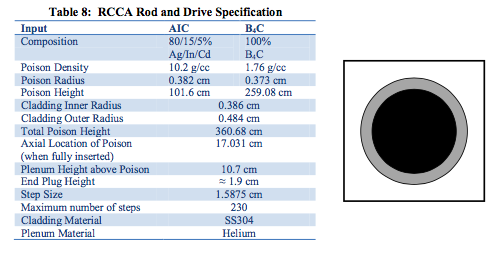
\includegraphics[scale=0.7]{Figures/Control Rod Geometries.png}
\end{figure}

\begin{figure}[htb!]
    \centering
    \subfloat{{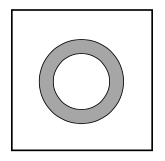
\includegraphics[width=5cm]{Figures/Instrument Thimble Geometry.png}}}%
    \qquad
    \subfloat{{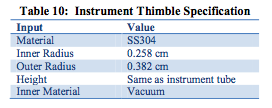
\includegraphics[width=9cm]{Figures/Instrument Thimble specs.png} }}%
\end{figure}

\begin{figure} [htb!]
\centering
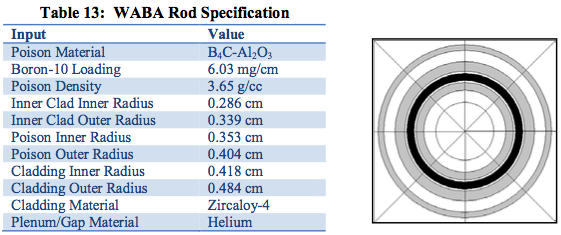
\includegraphics[scale=0.7]{Figures/WABA specs.png}
\end{figure}

\newpage
\thispagestyle{empty}

\begin{figure} [htb!]
\centering
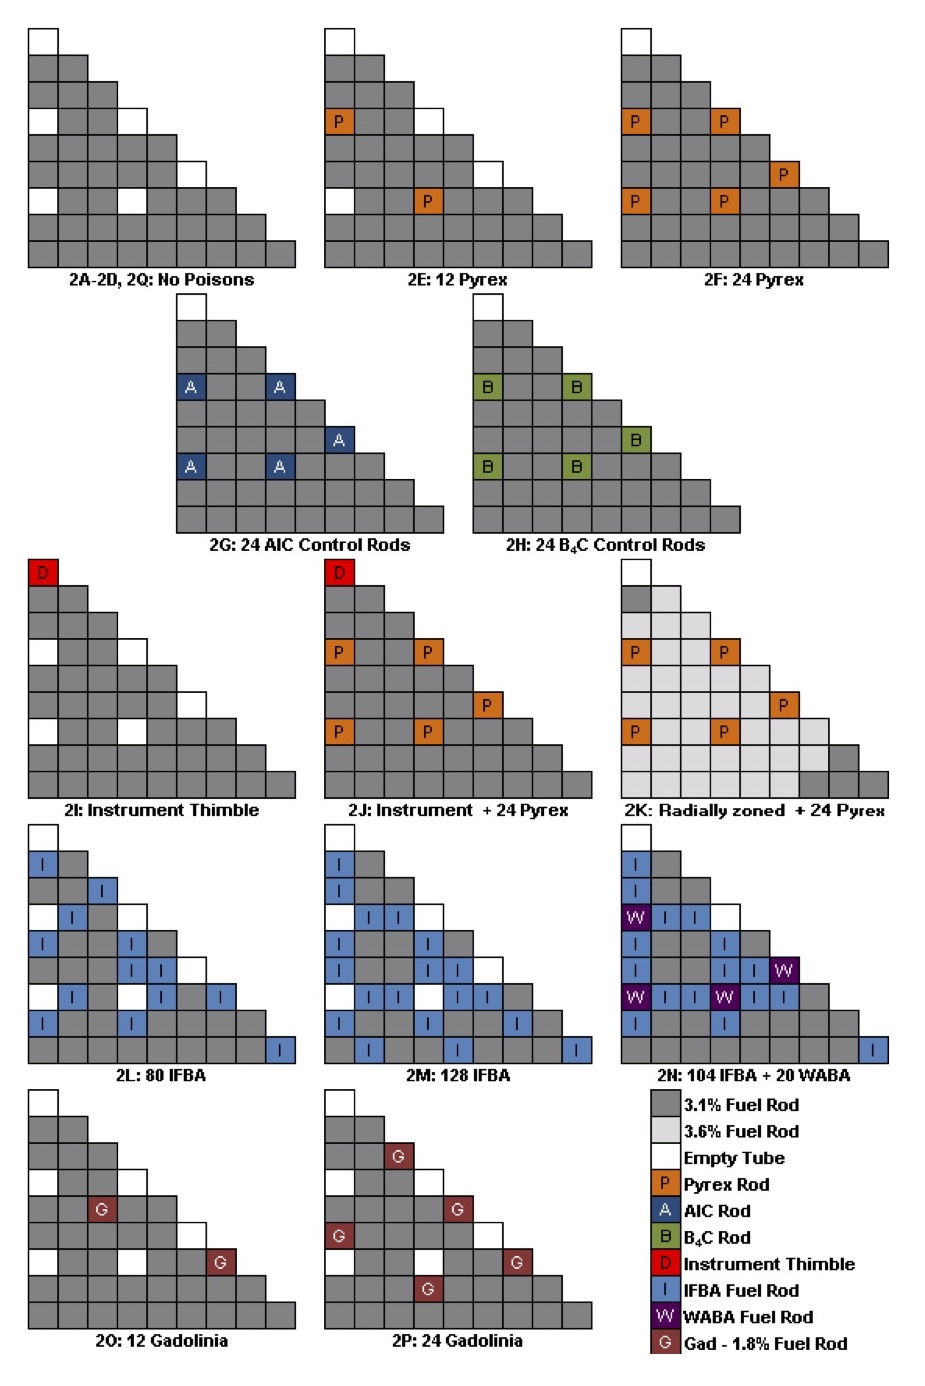
\includegraphics[scale=0.38]{Figures/assemblies.jpg}
\caption{CASL P2 Assembly Geometries}
\end{figure}

\clearpage


\section{Second Appendix: All graphable $K_{eff}$ results, Assembly A $K_{eff}$ burnup, Pin-Power Maps}

\thispagestyle{empty}

\begin{figure} [htb!]
\centering
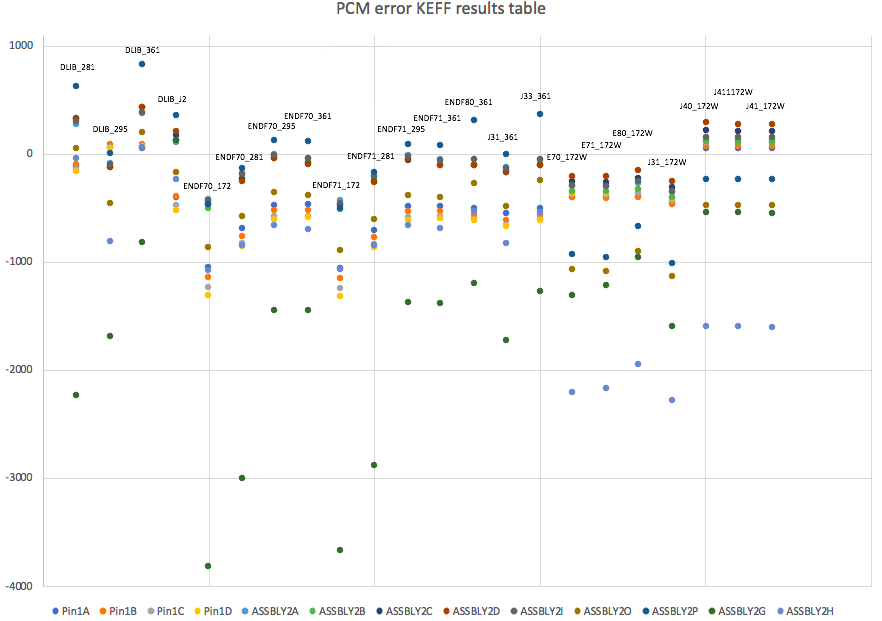
\includegraphics[scale=0.6]{Figures/allData1.png}
\caption{}
\end{figure}

\newpage

\thispagestyle{empty}

\begin{figure} [htb!]
\centering
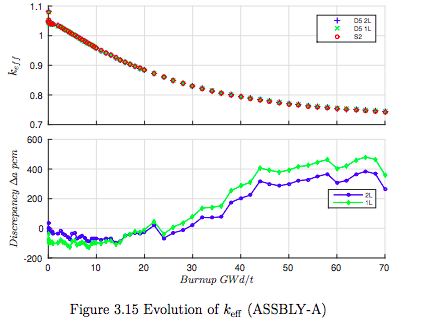
\includegraphics[scale=1.0]{Figures/Fig 3.15.png}
\end{figure}

\begin{figure}[htb!]

        \begin{subfigure}{.5\textwidth} % this sets the figure to be max half the width of the page
            \centering
            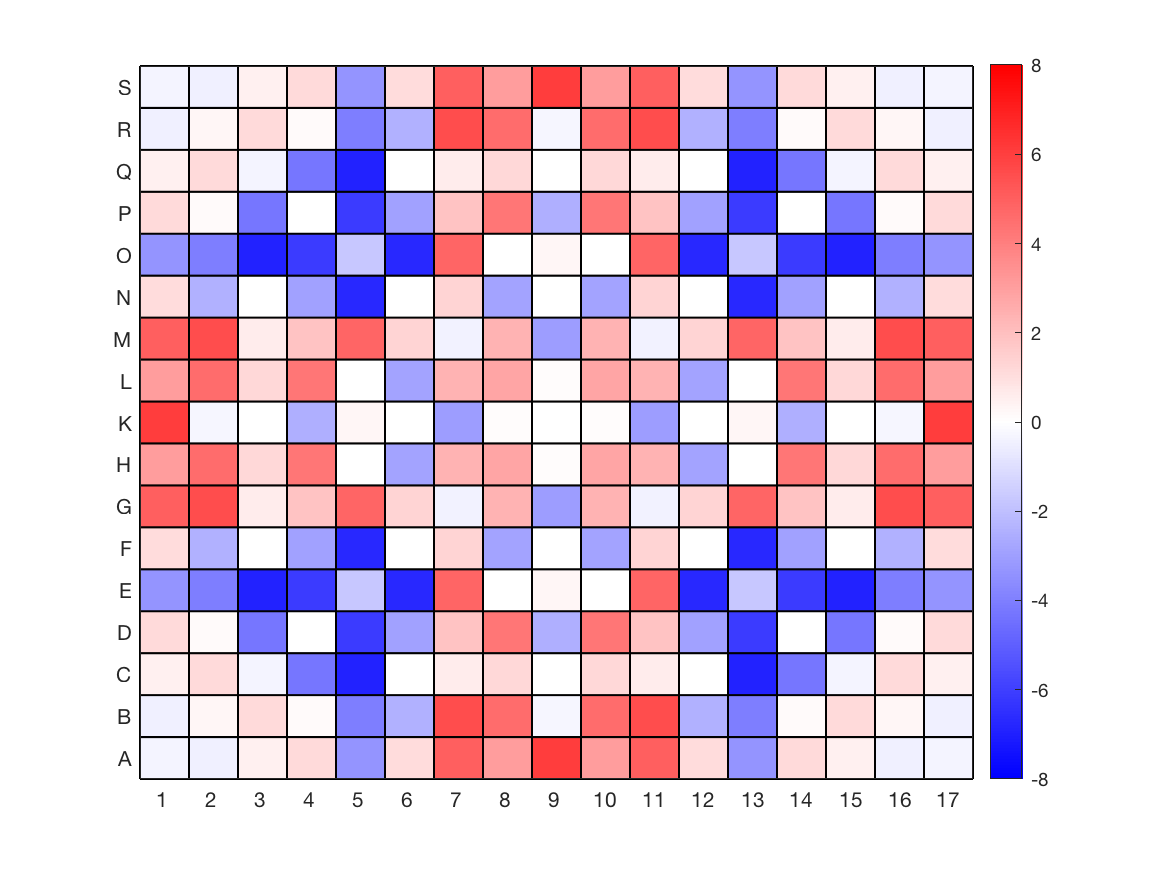
\includegraphics[scale=0.46]{Figures/2B_1L_pinpowerDiff.png} 
            \caption{Assembly 2B 1L Pin Power percent difference Map}
            \label{fig:sub-first}
        \end{subfigure}
        \begin{subfigure}{.5\textwidth}
            \centering
            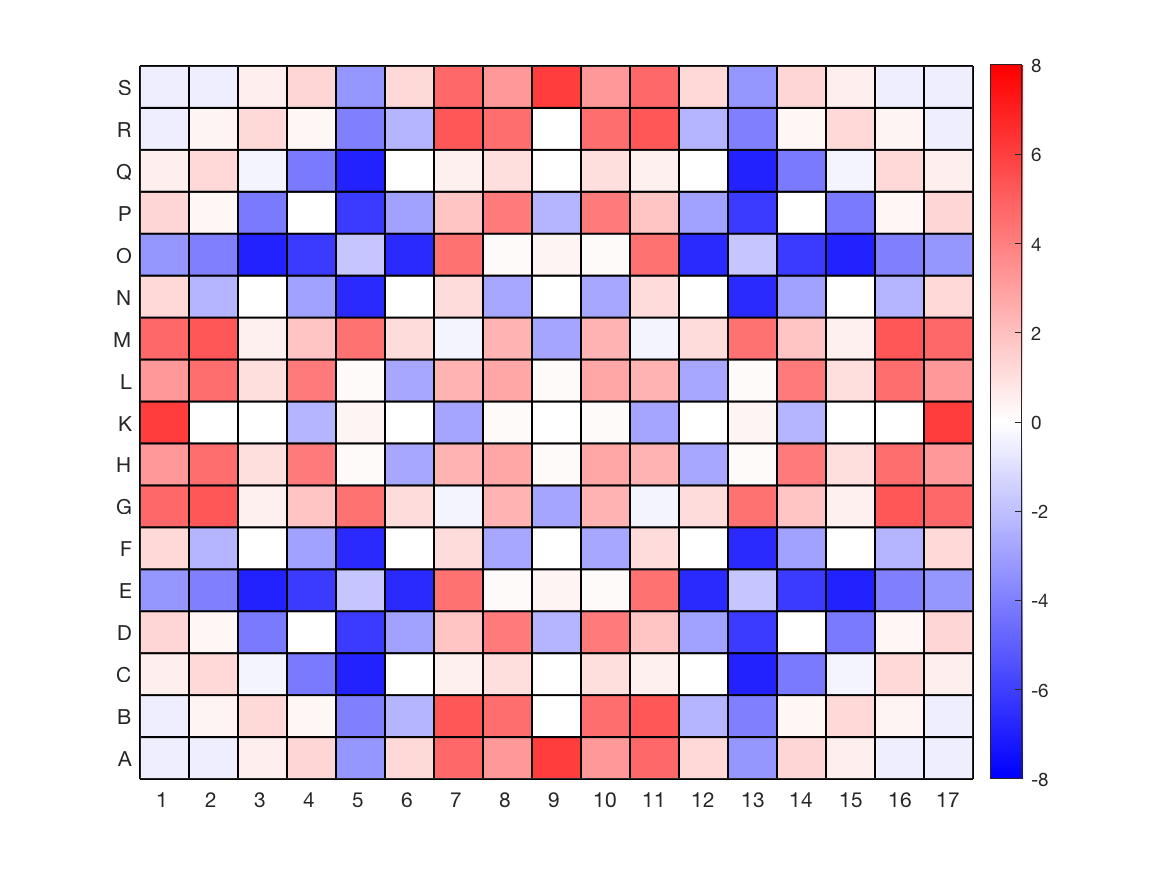
\includegraphics[scale=0.46]{Figures/2B_2L_pinpowerDiff.png} 
            \caption{Assembly 2B 2L Pin Power percent difference Map}
            \label{fig:sub-second}
        \end{subfigure}

        \label{fig:fig}
        \begin{subfigure}{\textwidth}
            \centering
            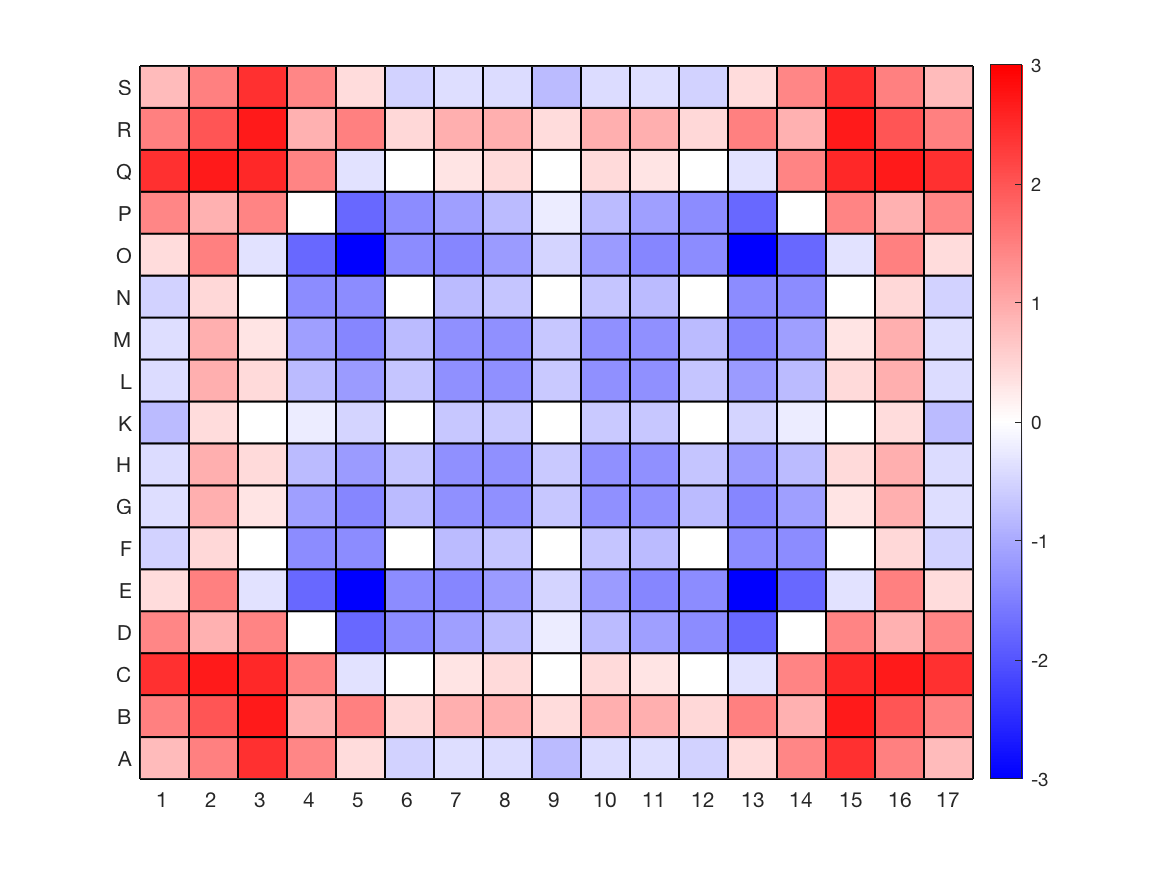
\includegraphics[scale=0.46]{Figures/2B_simple_pinpowerDiff.png}
            \caption{Assembly 2B Simple Pin Power percent difference Map}
            \label{fig:sub-firstA}
        \end{subfigure}
        \caption{Assembly 2B Pin Powers}
    \end{figure}
    
\newpage

\thispagestyle{empty}

\clearpage
\thispagestyle{empty}

\begin{figure}[htb!]

        \begin{subfigure}{.5\textwidth} % this sets the figure to be max half the width of the page
            \centering
            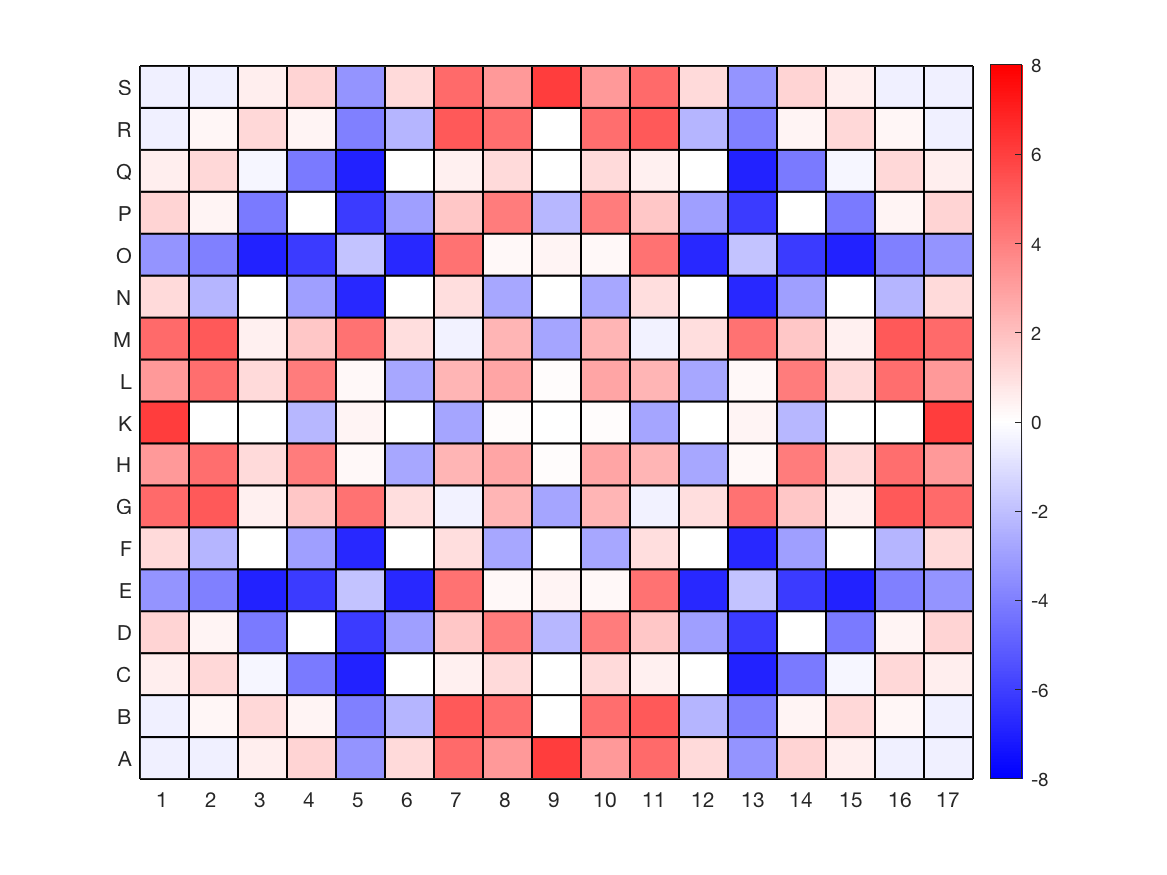
\includegraphics[scale=0.46]{Figures/2C_1L_pinpowerDiff.png} 
            \caption{Assembly 2C 1L Pin Power percent difference Map}
            \label{fig:sub-first}
        \end{subfigure}
        \begin{subfigure}{.5\textwidth}
            \centering
            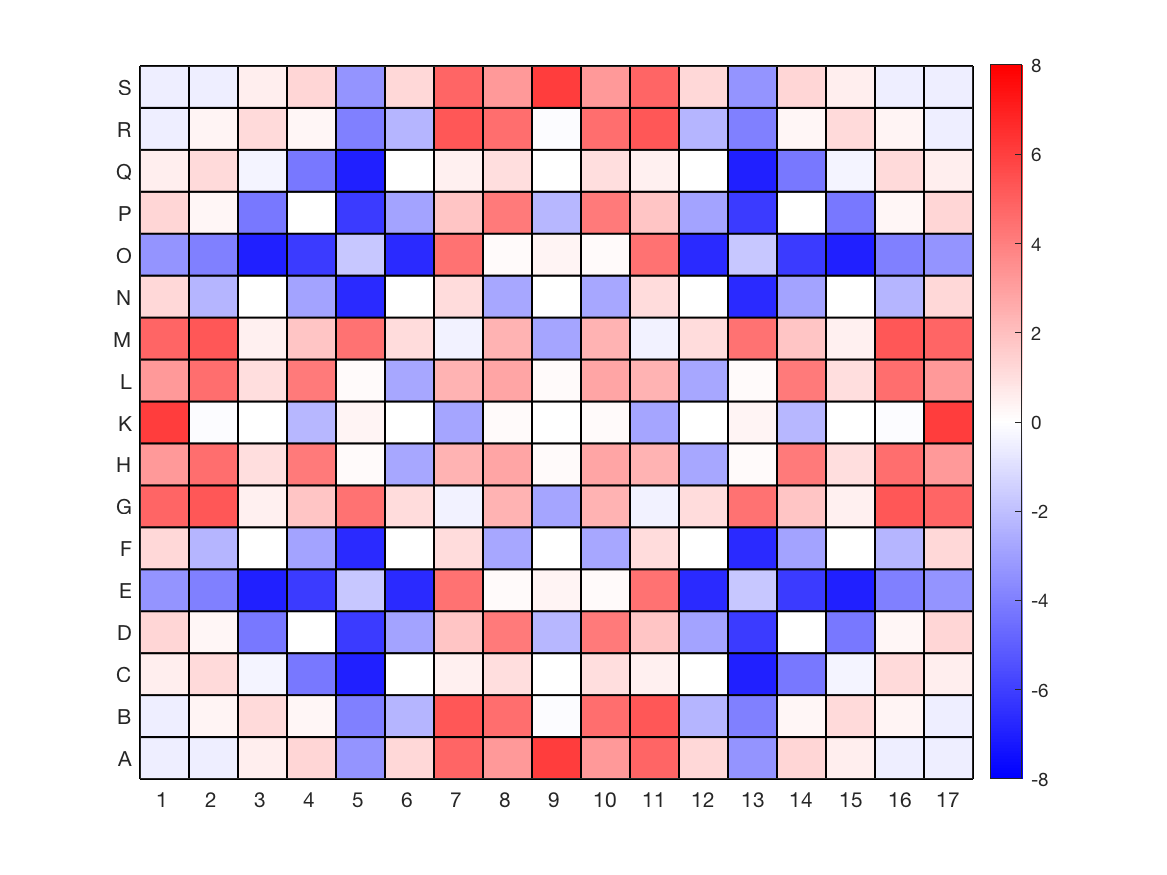
\includegraphics[scale=0.46]{Figures/2C_2L_pinpowerDiff.png} 
            \caption{Assembly 2C 2L Pin Power percent difference Map}
            \label{fig:sub-second}
        \end{subfigure}

        \label{fig:fig}
        \begin{subfigure}{\textwidth}
            \centering
            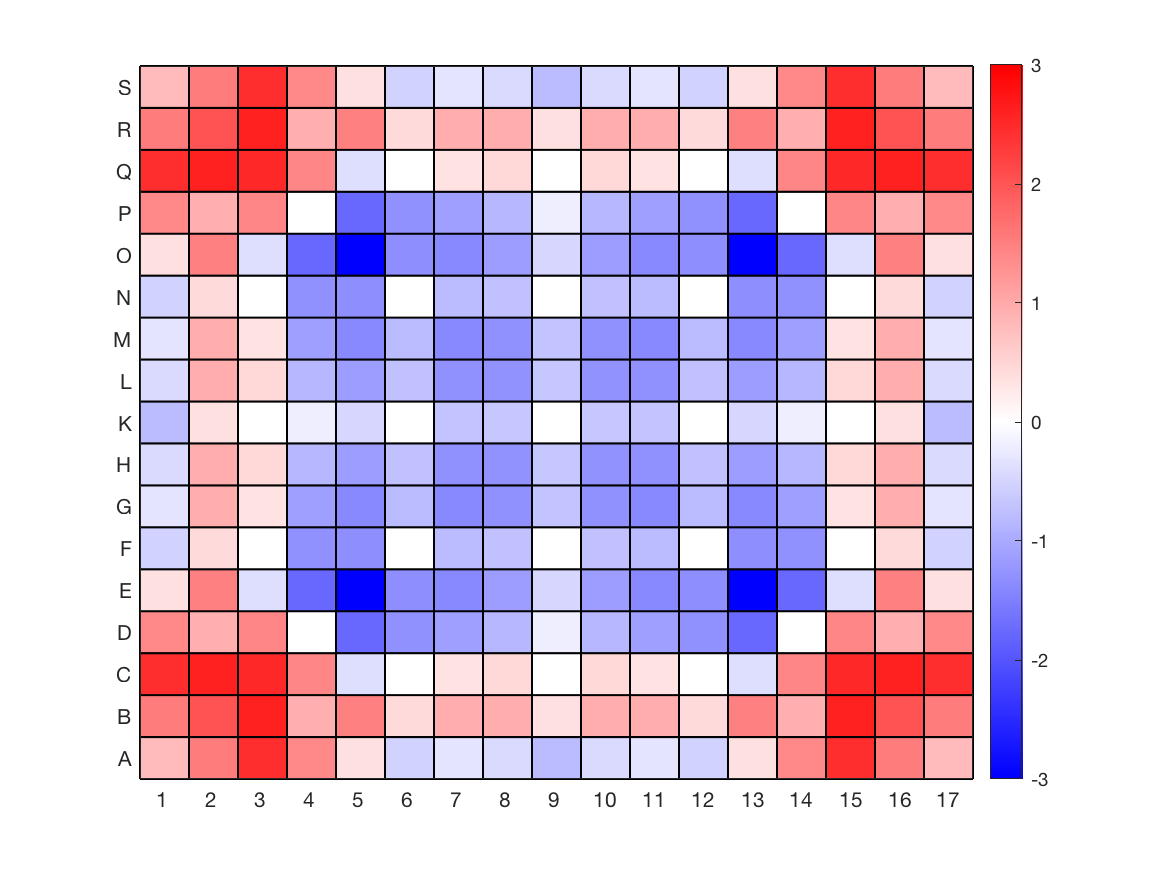
\includegraphics[scale=0.46]{Figures/2C_simple_pinpowerDiff.png}
            \caption{Assembly 2C Simple Pin Power percent difference Map}
            \label{fig:sub-firstA}
        \end{subfigure}
        \caption{Assembly 2C Pin Powers}
    \end{figure}
    
 
\clearpage
\thispagestyle{empty} 
    
\begin{figure}[htb!]

        \begin{subfigure}{.5\textwidth} % this sets the figure to be max half the width of the page
            \centering
            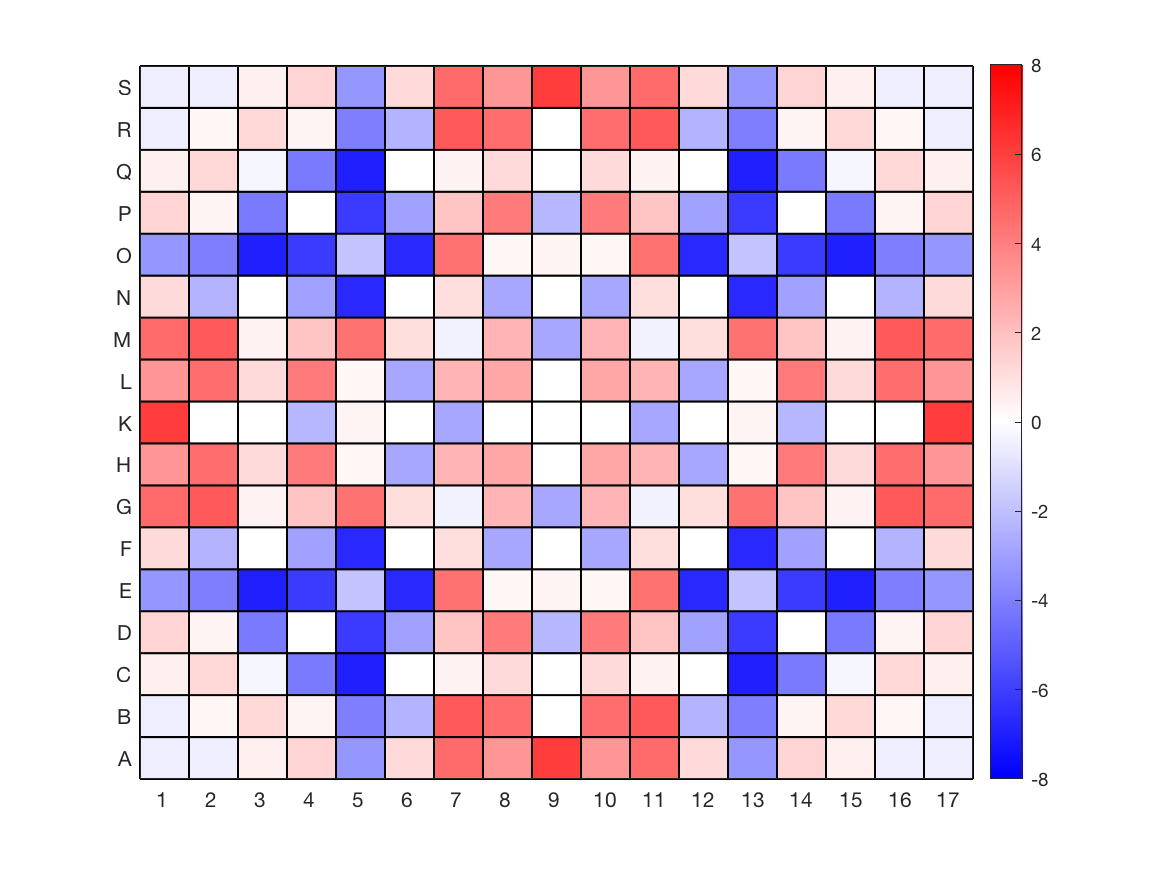
\includegraphics[scale=0.46]{Figures/2D_1L_pinpowerDiff.png} 
            \caption{Assembly 2D 1L Pin Power percent difference Map}
            \label{fig:sub-first}
        \end{subfigure}
        \begin{subfigure}{.5\textwidth}
            \centering
            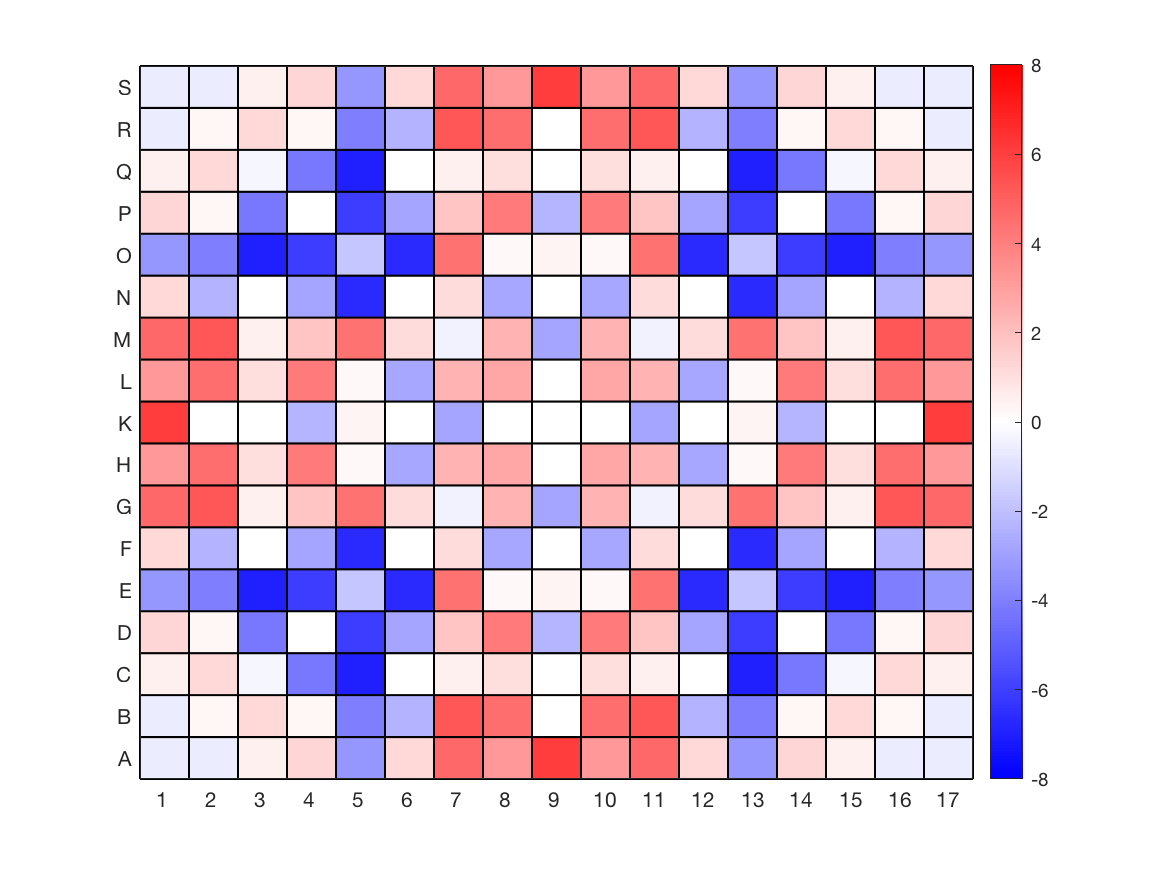
\includegraphics[scale=0.46]{Figures/2D_2L_pinpowerDiff.png} 
            \caption{Assembly 2D 2L Pin Power percent difference Map}
            \label{fig:sub-second}
        \end{subfigure}

        \label{fig:fig}
        \begin{subfigure}{\textwidth}
            \centering
            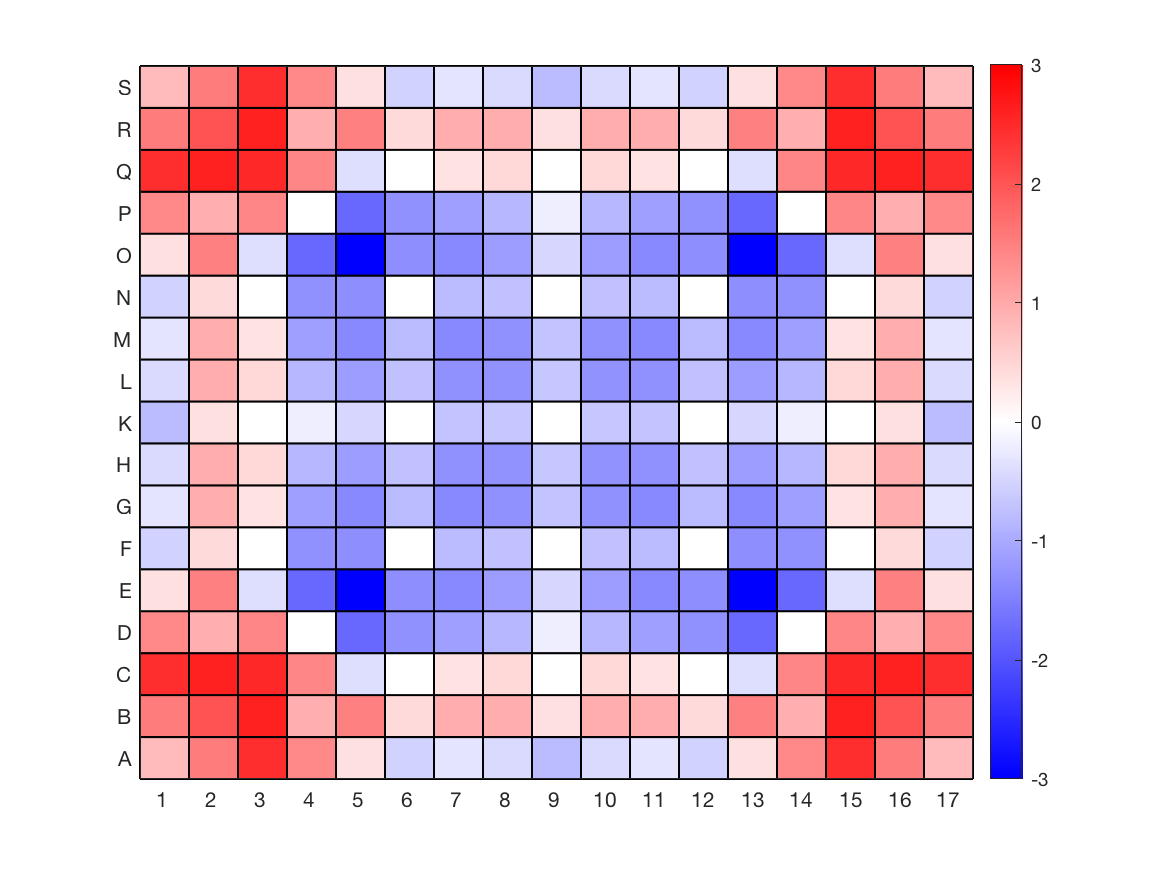
\includegraphics[scale=0.46]{Figures/2D_simple_pinpowerDiff.png}
            \caption{Assembly 2D Simple Pin Power percent difference Map}
            \label{fig:sub-firstA}
        \end{subfigure}
        \caption{Assembly 2D Pin Powers}
    \end{figure} 
    
 
 

\end{document}
